\documentclass[10pt,letterpaper,twocolumn]{article}
\usepackage[T1]{fontenc}
\usepackage[utf8]{inputenc}
\usepackage{times}
\usepackage{amsmath,amssymb}
\usepackage[letterpaper,margin=0.75in,columnsep=0.3in]{geometry}
\usepackage{graphicx}
\usepackage{booktabs}
\usepackage{caption}
\usepackage{titlesec}
\usepackage{enumitem}
\usepackage{xcolor}
\usepackage[hidelinks]{hyperref}

\captionsetup{font=small,labelfont=bf,labelsep=period}
\captionsetup[table]{position=top,skip=4pt}
\titleformat{\section}{\normalsize\scshape}{\thesection.}{0.5em}{}
\titleformat{\subsection}{\normalsize\bfseries}{\thesubsection}{0.5em}{}
\titlespacing*{\section}{0pt}{10pt}{5pt}
\titlespacing*{\subsection}{0pt}{8pt}{4pt}
\setlist{nosep,leftmargin=1.2em}
\renewcommand{\thesubsection}{\thesection.\arabic{subsection}}
\newcommand{\para}[1]{\textbf{#1}\hspace{0.4em}}

\begin{document}

\twocolumn[{%
\begin{center}
{\Large\bfseries Is Universal Computation Easy to Find? A Network View of\\[2pt] Elementary Cellular Automaton Rule Space\par}
\vspace{10pt}
\begin{minipage}[t]{0.45\textwidth}\centering
Dhiwakaran\footnotemark\\[1pt]
{\small Roll No.\ 22PT21}\\
{\small Dept.\ of Applied Mathematics and Computational Sciences}\\
{\small PSG College of Technology, Coimbatore, India}
\end{minipage}\hfill
\begin{minipage}[t]{0.45\textwidth}\centering
Ranjana\\[1pt]
{\small Roll No.\ 22PT25}\\
{\small Dept.\ of Applied Mathematics and Computational Sciences}\\
{\small PSG College of Technology, Coimbatore, India}
\end{minipage}\\[8pt]
November 2026\\[12pt]
\begin{minipage}{0.92\textwidth}
\small
\textbf{Abstract.} Akhlaghpour (2022) argues that cells may perform universal computation with RNA, and part of his case is that simple universal rule systems are easy for evolution to stumble on. We test that premise with network science on the smallest rule space that contains a proven universal system: the 256 elementary cellular automata (ECA), among them Rule~110. We simulate every rule, classify its behaviour automatically, and build the \emph{mutation network} in which two rules are linked when their rule tables differ in one bit, an 8-dimensional hypercube with 256 nodes and 1{,}024 edges. We find four things. (1) Behaviour is clustered in rule space: assortativity by class is 0.18, about 8 standard deviations above a shuffled-label null. (2) Complex behaviour is rare (4 of 256 rules: Rule~110 and its three symmetric twins) and isolated, yet no rule is more than 5 mutations away; this closeness is what the hypercube alone predicts. (3) Complex rules sit on the edge of chaos: 37.5\% of their neighbours are chaotic against 12.5\% overall ($p \approx 0.0002$). (4) Switched on from most to least irregular, rules percolate abruptly: the largest cluster stays at 13 rules until two borderline periodic rules bridge the chaotic fragments, and it jumps to 33 rules at 16\% occupation, ahead of the random-order curve. All results are identical across nine classifier settings, with Rule~54 counted as complex, and in a fresh simulation. As an application, we use these facts to search for a computation-capable rule with as few tests as possible: an edge-of-chaos search reduces the median number of rules tested from 41 to 23.\\[4pt]
\textbf{Keywords:} cellular automata, universal computation, rule space, mutation network, assortativity, percolation, edge of chaos, evolutionary search
\end{minipage}
\vspace{14pt}
\end{center}
}]
\footnotetext{Code and frozen analysis definitions are listed in Appendix~A and available from the authors.}

\section{Introduction}

Some very simple systems can compute anything a computer can. Rule~110, a one-dimensional cellular automaton whose rule fits in eight bits, is computationally universal~\cite{cook2004}. Akhlaghpour~\cite{akhlaghpour2022} uses this kind of observation in a biological argument. He notes that network models of the brain and the cell (neural, gene-regulatory and signalling networks) have bounded memory and are not known to be universal, and proposes that cells may instead compute with RNA, whose editing operations can implement universal combinatory logic. One step in his argument is that simple universal rule sets are easy to stumble upon, so evolution would plausibly have found one.

That step is a claim about the \emph{space of rules} and how it is explored. Evolution changes rules by small mutations, so whether universality is easy to find depends on where computation-capable rules sit relative to all others, and on whether they can be reached one mutation at a time. These are questions about paths and clusters in a network.

We study the smallest rule space that contains a proven universal system: the 256 elementary cellular automata (ECA). We ask five research questions:
\begin{itemize}
\item \textbf{RQ1.} Is behaviour organised in rule space, that is, do rules with similar behaviour sit next to each other?
\item \textbf{RQ2.} Where are the complex rules: how far are they from other rules, how isolated are they, and what lies around them?
\item \textbf{RQ3.} Do the irregular (chaotic and complex) rules percolate into one connected cluster, and does this differ from random occupation?
\item \textbf{RQ4.} Are the findings robust to classification thresholds, to borderline rules, and to the simulation itself?
\item \textbf{RQ5.} Can these facts make the search for a computation-capable rule cheaper?
\end{itemize}

\para{Contributions.} (1) A complete, automatically classified mutation network of the ECA rule space, with every measure compared against a shuffled-label null model. (2) Quantitative evidence that complex rules are rare, isolated and adjacent to chaos, separating effects of the class layout from properties of the hypercube itself. (3) A percolation analysis showing that irregular rules connect abruptly through a few borderline rules. (4) A search experiment that turns the edge-of-chaos result into a practical heuristic for finding rare, computation-capable designs.

\section{Related Work}

\para{Universal computation in simple systems.} Wolfram sorted cellular automata into four classes (fixed, periodic, chaotic and complex) and conjectured that complex rules support universal computation~\cite{wolfram1984}. Cook proved Rule~110 universal through colliding gliders~\cite{cook2004}. Akhlaghpour~\cite{akhlaghpour2022} connects this line of work to biology, proposing RNA as a substrate for natural universal computation.

\para{Rule space and the edge of chaos.} Langton introduced the parameter $\lambda$, the share of non-quiescent outputs in a rule table, and argued that computation occurs at a transition between order and chaos~\cite{langton1990}. Li and Packard studied the ECA rule space directly, linking rules by Hamming distance and mapping where each class lies~\cite{lipackard1990}. Mitchell, Hraber and Crutchfield found that evolved CA do not always sit at the edge of chaos and criticised overly broad readings of the idea~\cite{mitchell1993}. We revisit Li and Packard's construction with network measures and explicit null models.

\para{Genotype networks and evolvability.} Schuster and colleagues showed that RNA sequences folding into the same shape form large neutral networks, so new shapes are often a few mutations away~\cite{schuster1994}. Wagner argued that such networks reconcile robustness with evolvability~\cite{wagner2008}. Weinreich and colleagues measured all $2^5$ combinations of five resistance mutations in a $\beta$-lactamase, a 5-cube genotype space, and found that few mutational paths are accessible~\cite{weinreich2006}. Our mutation network applies the same lens to rule tables.

\para{Network measures.} We use assortative mixing~\cite{newman2003}, shortest paths, and site percolation~\cite{stauffer1994,callaway2000}. On the $n$-dimensional hypercube, the giant component appears at an occupation of order $1/n$~\cite{ajtai1982}. Compression has been used to classify CA behaviour~\cite{zenil2010}; we use it as one of our behaviour measures.

\section{Data}

\para{Rule space.} An ECA updates each cell of a row from its own state and its two neighbours. The eight possible neighbourhoods each map to an output bit, so a rule is an 8-bit string and there are $2^8 = 256$ rules, named by the decimal value of the string (Wolfram's convention). Rule~110 is \texttt{01101110}.

\para{Simulation.} Every rule is run from 5 random initial rows of 200 cells with periodic boundaries for 1{,}200 steps. Random rows use a fixed seed. From each run we record:
\begin{itemize}
\item \emph{Uniform}: whether the final row is all 0s or all 1s.
\item \emph{Periodicity and transient}: the first step at which a row repeats an earlier row up to a cyclic shift, and the period.
\item \emph{Compressibility}: the zlib compression ratio of the last 400 rows, divided by that of random bits of the same size, so that noise scores about 1 and order scores near 0.
\item \emph{Damage}: the fraction of cells that differ after 150 steps when one initial cell is flipped.
\end{itemize}
Measures are averaged over the 5 runs. Figure~\ref{fig:examples} shows typical behaviour.

\begin{figure*}[t]
\centering
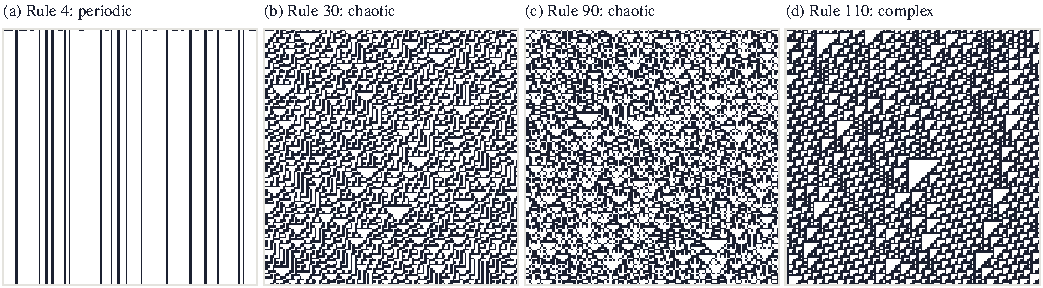
\includegraphics[width=\textwidth]{figures/fig_examples.pdf}
\caption{Space-time diagrams from one random initial row of 120 cells (time runs downward). (a) Rule~4 settles into stable stripes. (b), (c) Rules 30 and 90 are chaotic. (d) Rule~110 shows moving structures that collide, the mechanism behind its universality.}
\label{fig:examples}
\end{figure*}

\section{Methods}

\subsection{Classification}
Each rule receives one of Wolfram's four classes using fixed thresholds (Appendix~A). Class~1 (\emph{fixed}): the final row is uniform in at least 60\% of runs. Class~2 (\emph{periodic}): otherwise, the pattern repeats in at least 60\% of runs within 600 steps. Class~4 (\emph{complex}): otherwise, the normalised compression ratio is below 0.4, meaning a long-lived but structured pattern. Class~3 (\emph{chaotic}): all remaining rules. Both cut-offs sit in wide empty gaps: no rule has a transient between 304 and 872 steps, and no rule has a compression ratio between 0.234 and 0.613. Section~\ref{sec:rq4} varies them.

\subsection{Mutation network}
Let $G=(V,E)$ with $V=\{0,\dots,255\}$ and $(u,v)\in E$ when the rule tables of $u$ and $v$ differ in exactly one bit, i.e.\ $v = u \oplus 2^k$ for some $k\in\{0,\dots,7\}$. One edge is one mutation. $G$ is the 8-dimensional hypercube $Q_8$: 256 nodes, 1{,}024 edges, every node of degree 8. Because $G$ is regular and vertex-transitive, any structure we find comes from where the classes are placed, not from the graph.

\subsection{Network measures}
\para{Assortativity (RQ1).} Newman's assortativity coefficient for categorical labels~\cite{newman2003},
\begin{equation}
r = \frac{\sum_i e_{ii} - \sum_i a_i^2}{1 - \sum_i a_i^2},
\end{equation}
where $e_{ij}$ is the fraction of edge ends joining class $i$ to class $j$ and $a_i=\sum_j e_{ij}$. We also report the mixing matrix: for rules of class $i$, the share of their neighbours in class $j$.

\para{Distance and isolation (RQ2).} For every rule, the shortest-path distance (number of mutations) to the nearest complex rule; for complex rules, the distance to the nearest \emph{other} complex rule; and the size of the largest connected cluster within each class.

\para{Neighbourhood enrichment (RQ2).} The share of chaotic rules among the $4\times 8 = 32$ neighbours of complex rules, compared with the share among all rules.

\para{Null model.} We keep $G$ fixed and randomly permute class labels across nodes, preserving class sizes. Assortativity uses 500 permutations, distances and cluster sizes 1{,}000 to 5{,}000, and the enrichment test 20{,}000. One-sided $p$-values are the share of permutations at least as extreme as the observed value.

\subsection{Percolation (RQ3)}
We switch nodes on one at a time and track the largest connected cluster of switched-on nodes, as a fraction of all 256 rules, at occupation fractions $f = 0.02, 0.04, \dots, 1$. Two orders are compared: \emph{irregular first}, ranking rules by decreasing compression ratio (so the 32 chaotic rules come first, then the 4 complex rules, then the most irregular periodic rules), and \emph{random order} (200 random orders, mean $\pm$ 2 s.d.). The seed-to-seed standard deviation of the random curve marks the finite-size crossover~\cite{stauffer1994}.

\subsection{Robustness (RQ4)}
We repeat the RQ1--RQ2 measures (i) under nine classifier settings, combining compression cut-offs $\{0.3, 0.4, 0.5\}$ with periodicity cut-offs $\{400, 600, 800\}$ steps; (ii) with Rule~54 and its mirror image Rule~147 counted as complex, since Rule~54 is often treated as a complex rule in the literature; and (iii) on a fresh simulation with a different random seed and 300 cells.

\section{Results}

\begin{table}[t]
\caption{Behaviour classes of the 256 ECA (means over rules in each class; compression: noise $\approx 1$; transient capped at 1{,}201 steps).}
\label{tab:classes}
\centering\small
\begin{tabular}{@{}lrrrr@{}}
\toprule
Class & Rules & Compr. & Transient & Damage \\
\midrule
1 Fixed & 24 & 0.003 & 6 & 0.00 \\
2 Periodic & 196 & 0.052 & 19 & 0.02 \\
3 Chaotic & 32 & 0.893 & 1{,}201 & 0.30 \\
4 Complex & 4 & 0.203 & 1{,}119 & 0.23 \\
\bottomrule
\end{tabular}
\end{table}

\subsection{Classification: complex behaviour is rare}
Table~\ref{tab:classes} gives the classes. Two measures separate them. Periodic rules repeat within at most 304 steps, while complex rules have not repeated after 872--1{,}201 steps; and complex rules compress to 0.18--0.23, far below chaotic rules (0.61--1.00). Only four rules are complex: 110, 124, 137 and 193. They are Rule~110 and its mirror image (124), colour-swap (137) and both (193), the family Cook proved universal~\cite{cook2004}. The classifier found this family without any rule being labelled by hand.

\begin{figure*}[t]
\centering
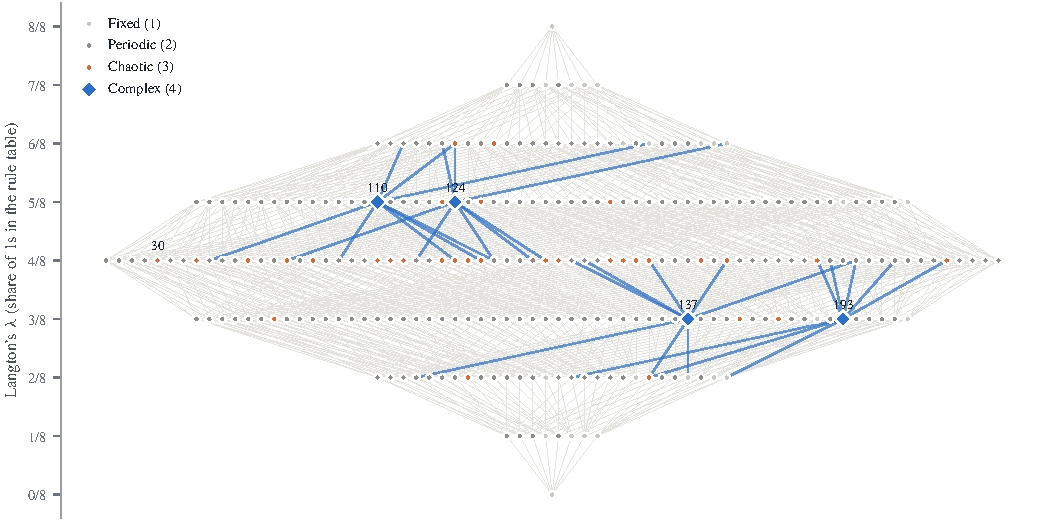
\includegraphics[width=\textwidth]{figures/fig_rulespace.pdf}
\caption{The mutation network of all 256 ECA. Rows group rules by Langton's $\lambda$; grey lines are the 1{,}024 single mutations; blue diamonds are the four complex rules and blue lines their eight mutations each. Chaotic and complex rules occupy the middle rows.}
\label{fig:rulespace}
\end{figure*}

\subsection{RQ1: Behaviour is clustered in rule space}
Figure~\ref{fig:rulespace} shows the network. Rules of the same class are neighbours far more often than chance. Assortativity by class is $r = 0.177$, against $-0.005 \pm 0.023$ under the null (about 8 standard deviations); 68.0\% of edges join rules of the same class against 60.9\% expected ($p < 0.001$).

\begin{table}[t]
\caption{Mixing matrix: for rules of each class (rows), the share of their eight neighbours in each class (columns).}
\label{tab:mixing}
\centering\small
\begin{tabular}{@{}lrrrr@{}}
\toprule
From $\backslash$ to & Fixed & Periodic & Chaotic & Complex \\
\midrule
Fixed & \textbf{0.417} & 0.521 & 0.042 & 0.021 \\
Periodic & 0.064 & \textbf{0.806} & 0.120 & 0.010 \\
Chaotic & 0.031 & 0.734 & \textbf{0.188} & 0.047 \\
Complex & 0.125 & 0.500 & 0.375 & \textbf{0.000} \\
\midrule
All rules & 0.094 & 0.766 & 0.125 & 0.016 \\
\bottomrule
\end{tabular}
\end{table}

Table~\ref{tab:mixing} shows where the clustering comes from. Fixed rules keep their class under 41.7\% of mutations against a base rate of 9.4\%, and chaotic rules 18.8\% against 12.5\%. The fixed rules form a cluster of 12 against 4.9 expected ($p=0.005$); the largest chaotic cluster has 13 rules against 7.6 expected ($p=0.08$). The landscape is nevertheless rugged: the compression scores of neighbouring rules are almost uncorrelated (Pearson $r = 0.07$), so there is no smooth gradient towards complexity.

\subsection{RQ2: Complex rules are isolated, close to everything, and border chaos}

\begin{table}[t]
\caption{Network measures against the shuffled-label null model.}
\label{tab:measures}
\centering\small
\begin{tabular}{@{}lrrr@{}}
\toprule
Measure & Observed & Null & $p$ \\
\midrule
Assortativity $r$ & 0.177 & $-0.005$ & $<0.001$ \\
Same-class edges & 68.0\% & 60.9\% & $<0.001$ \\
Complex--complex edges & 0 & -- & -- \\
Nearest other complex & 2.00 & 2.85 & 0.14 \\
Mean distance to complex & 2.61 & 2.56 & 0.71 \\
Chaotic share next to complex & 37.5\% & 12.5\% & 0.0002 \\
\bottomrule
\end{tabular}
\end{table}

\para{Isolated islands.} No two complex rules are neighbours: each is exactly two mutations from the nearest other complex rule (Table~\ref{tab:measures}). This follows from symmetry. A mirror image swaps the outputs of neighbourhood pairs such as \texttt{001} and \texttt{100}, so when it changes a rule it changes at least two bits.

\para{Never far, as the hypercube predicts.} Of the 256 rules, 116 (45\%) are within two mutations of a complex rule, and all are within five (mean 2.61). This closeness is not special to complex rules: four nodes placed at random in $Q_8$ give a mean distance of 2.56 ($p=0.71$). In a hypercube, a small target set is always close. For Akhlaghpour's argument this cuts both ways: universality is never far away, but nothing in the layout leads towards it.

\begin{figure}[t]
\centering
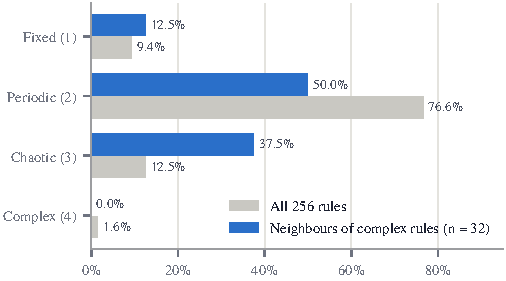
\includegraphics[width=\columnwidth]{figures/fig_neighbours.pdf}
\caption{Class composition of all rules (grey) and of the 32 neighbours of complex rules (blue). Chaotic rules are three times over-represented next to complex rules.}
\label{fig:neighbours}
\end{figure}

\para{On the edge of chaos.} The layout does single out what surrounds complex rules. Of their 32 neighbours, 12 (37.5\%) are chaotic, three times the 12.5\% base rate; in 20{,}000 label permutations a share this high occurred 4 times ($p \approx 0.0002$; Figure~\ref{fig:neighbours}). Every complex rule has exactly three chaotic neighbours. Complex rules also sit at $\lambda = 3/8$ or $5/8$, beside the chaotic band at the centre of Figure~\ref{fig:rulespace}. Langton's edge-of-chaos idea~\cite{langton1990} therefore appears here as a measurable property of the mutation network.

\subsection{RQ3: Irregular rules percolate abruptly}

\begin{figure}[t]
\centering
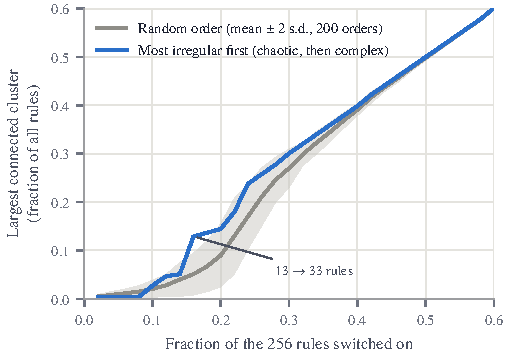
\includegraphics[width=\columnwidth]{figures/fig_percolation.pdf}
\caption{Largest connected cluster as rules are switched on. Grey: random order (200 orders, band $\pm 2$ s.d.). Blue: most irregular first. Two borderline periodic rules bridge the chaotic fragments at 15--16\% occupation.}
\label{fig:percolation}
\end{figure}

\para{Random occupation.} With rules switched on in random order, the largest cluster grows smoothly, rising most steeply between $f=0.20$ and $0.26$ (Figure~\ref{fig:percolation}). The order-to-order standard deviation peaks at $f=0.22$, the usual finite-size marker of a percolation crossover. On $Q_n$ the giant component appears at an occupation of order $1/n$~\cite{ajtai1982}, here $1/8$; at $n=8$, finite size moves the observed crossover higher.

\para{Irregular first.} Ranked by irregularity, the first 32 rules switched on are the chaotic rules. They form 12 separate fragments, the largest of 13 rules (5.1\% of all rules). The four complex rules come next (ranks 33--37) and connect none of them. The jump comes from two borderline periodic rules, the most irregular of their class: Rule~181 (compression 0.148) links the largest fragment to others and the cluster grows to 23 rules; Rule~82 (0.137) brings it to 33 rules (12.9\%) at $f=0.16$. At that point the random-order cluster is $5.1\% \pm 2.2\%$, so the irregular-first curve lies about 3.5 standard deviations above it. It stays above the random band at $f=0.16$--$0.18$ and merges with it from $f \approx 0.20$, once ordinary periodic rules dominate both orders.

\para{Interpretation.} The irregular region of rule space is not one connected piece. It is a set of fragments that a few borderline rules join suddenly. A population drifting through chaotic rules could therefore stay trapped in one fragment until a rare bridging mutation opens the next.

\subsection{RQ4: The results are robust}
\label{sec:rq4}

\begin{table}[t]
\caption{Robustness of the main measures (complex rules, assortativity $r$ with its $z$-score against the null, chaotic share next to complex rules).}
\label{tab:robust}
\centering\small\setlength{\tabcolsep}{4pt}
\begin{tabular}{@{}lrrrr@{}}
\toprule
Setting & Cmplx & $r$ & $z$ & Chaotic nb. \\
\midrule
Main (0.4, 600) & 4 & 0.177 & 7.9 & 37.5\% \\
9 threshold settings & 4 & 0.177 & 7.8--8.7 & 37.5\% \\
Rule 54 as complex & 6 & 0.170 & 7.7 & 33.3\% \\
Fresh simulation & 4 & 0.177 & 8.0 & 37.5\% \\
\bottomrule
\end{tabular}
\end{table}

All nine classifier settings produce the same four complex rules and identical network measures (Table~\ref{tab:robust}); only the $z$-scores vary, because they depend on the random permutations. The measures fall in wide gaps, so the thresholds do not matter within these ranges. Counting Rule~54 and its mirror image as complex leaves every conclusion intact: complex rules still have no complex neighbours, and chaotic rules are still enriched next to them (33.3\% against 11.7\%, $p<0.001$). A fresh simulation with a different seed (7) and a wider lattice (300 cells) assigns every one of the 256 rules to the same class.

\section{Application: Finding a Computation-Capable Rule with Few Tests}

\para{The problem.} Many design problems share one structure: a large space of candidate rules or designs, a few of which have a rare, valuable property, and an expensive test for that property. Examples include searching chemical or molecular rule systems that can compute, as Akhlaghpour's theory implies evolution did; designing gene-regulatory or synthetic-biology circuits with a target behaviour; and anticipating which mutations bring a pathogen enzyme to drug resistance, where genotypes also form a hypercube~\cite{weinreich2006}. In each case, testing a candidate costs a simulation, an experiment or a synthesis. The goal is to find a target with as few tests as possible. We pose this problem on ECA rule space, where ground truth is known: find a complex rule, counting the number of distinct rules tested.

\para{Strategies.} Each search starts from a random rule; we run 20{,}000 searches per strategy.
\begin{itemize}
\item \emph{Random testing}: test rules in random order, using no structure.
\item \emph{Blind mutation walk}: a random walk on $G$, testing every rule visited.
\item \emph{$\lambda$-guided}: random testing restricted to the middle rows, $\lambda \in \{3/8, 4/8, 5/8\}$ (182 rules), the band where Figure~\ref{fig:rulespace} places irregular behaviour.
\item \emph{Edge-of-chaos walk}: a blind walk until a chaotic rule is found; then test all eight neighbours of every chaotic rule reached, expanding the chaotic region breadth-first (RQ2); resume the blind walk if that region is used up.
\item \emph{Combined}: $\lambda$-guided testing until a chaotic rule is found, then edge-of-chaos expansion.
\end{itemize}

\begin{table}[t]
\caption{Rules tested until a complex rule is found (20{,}000 searches per strategy; mean $\pm$ s.e., median, 90th percentile, share of searches done within 20 tests).}
\label{tab:search}
\centering\small\setlength{\tabcolsep}{3.5pt}
\begin{tabular}{@{}lrrrr@{}}
\toprule
Strategy & Mean & Med. & P90 & $\le$20 \\
\midrule
Random testing & $51.3 \pm 0.3$ & 41 & 111 & 27.6\% \\
Blind mutation walk & $51.1 \pm 0.3$ & 41 & 112 & 28.4\% \\
$\lambda$-guided & $\mathbf{36.5 \pm 0.2}$ & 29 & \textbf{79} & 37.5\% \\
Edge-of-chaos walk & $44.5 \pm 0.3$ & 26 & 98 & 42.9\% \\
Combined & $42.7 \pm 0.3$ & \textbf{23} & 92 & \textbf{45.5\%} \\
\bottomrule
\end{tabular}
\end{table}

\begin{figure}[t]
\centering
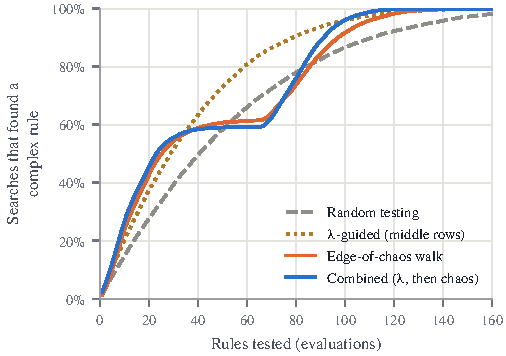
\includegraphics[width=\columnwidth]{figures/fig_search.pdf}
\caption{Share of searches that have found a complex rule after a given number of tests. Network-guided searches finish early more often (vertical line: 20 tests); the plateau between about 35 and 65 tests comes from searches that explore the 13-rule chaotic cluster, which borders no complex rule.}
\label{fig:search}
\end{figure}

\para{Findings.} Random testing needs 51.3 tests on average, matching the exact value $(256+1)/(4+1) = 51.4$ (Table~\ref{tab:search}). A blind mutation walk is no better: in a hypercube, mutating at random is as good as sampling at random. Using the network results helps. The edge-of-chaos walk cuts the median from 41 to 26 tests and raises the share of searches that succeed within 20 tests from 27.6\% to 42.9\%; the combined strategy reaches a median of 23 (44\% fewer tests) and 45.5\%.

The mean improves less, from 51.3 to 42.7, and here the $\lambda$-guided strategy is best (36.5). The reason is visible in Figure~\ref{fig:search} and in the cluster structure from RQ3: only 6 of the 12 chaotic fragments, holding 14 of the 32 chaotic rules, touch a complex rule. The largest fragment, with 13 rules, touches none. A search that enters it spends many tests before leaving, which produces the plateau in Figure~\ref{fig:search}. The edge-of-chaos heuristic is therefore excellent when it lands in the right fragment and costly when it does not.

\para{What this solves.} The network view turns a needle-in-a-haystack search into a guided one: look where chaos is, then test its neighbours. It also shows the limit of the heuristic: chaos is necessary but not sufficient. A practical design would stop expanding a chaotic region after a fixed budget, or combine the $\lambda$ prior with the neighbourhood rule as our combined strategy does.

\section{Discussion}

\para{Rare, isolated and near chaos.} In the smallest rule space with a universal rule, complex behaviour is rare (1.6\% of rules) and sits in isolated islands, but always within a few mutations and always beside chaotic rules. These three facts have different origins. The closeness is a property of the hypercube; the isolation comes from the symmetry of the Rule~110 family; the adjacency to chaos is a genuine feature of where behaviour lies, which no relabelling of the space reproduces.

\para{What this means for Akhlaghpour's premise.} The premise that universal rules are easy to stumble on is supported in a specific sense. A random walker finds a complex rule after about 51 tests, the same as random sampling; nothing is hidden or hard to reach. A walker that follows chaos does better. But the landscape offers no smooth gradient (neighbouring complexity is uncorrelated), and the chaotic region is fragmented, so evolution would reach universality by drift and by chance bridges rather than by steady improvement. Whether this holds in the far larger rule spaces of real molecular systems is open; our results show what to measure there.

\para{Connectivity versus usefulness.} The percolation analysis separates two questions that are easy to conflate. The irregular part of rule space does connect up as rules are added, and earlier than random. But connection alone does not make complexity reachable: the search experiment shows that one large chaotic fragment leads nowhere. Network position therefore helps, but it must be combined with knowing which fragment borders the target.

\para{Beyond cellular automata.} The method needs only a rule or genotype space, a mutation operator and a behaviour label, so it transfers directly. In protein and RNA design~\cite{schuster1994}, and in drug-resistance genotype spaces~\cite{weinreich2006}, the same measures (assortativity of function, distance to function, enrichment of neighbours and percolation of functional genotypes) would show how findable a rare function is and which neighbouring states signal it.

\section{Limitations}

\para{Small rule space.} 256 rules make every measure exact but limit statistical power and make the percolation curve stepped. Larger spaces, such as ECA with radius 2 or small Turing machines, would sharpen the transition.

\para{Complex is a proxy for universal.} Only Rule~110 and its symmetric twins are proven universal. Our class~4 is defined by behaviour (long transients and structured patterns), not by a proof of universality.

\para{Classification.} Behaviour is measured from finite runs of 200 cells and 1{,}200 steps. Thresholds were fixed before the network analysis, and the measures sit in wide gaps that make them insensitive to the exact values (RQ4), but borderline rules such as Rule~54 remain debatable.

\para{Mutation model.} We treat one bit flip as one mutation with all flips equally likely. Real mutation operators on molecular rules may be biased or change several outputs at once.

\para{Exploratory decisions.} The percolation ordering (by compression score) and the strategies in Section~6 were chosen after the RQ1--RQ2 results; we list them in Appendix~A.

\section{Conclusion}

We built the mutation network of all 256 elementary cellular automata and asked whether computation-capable rules are easy to find. Behaviour is clustered in rule space (assortativity 0.18, $z \approx 8$). Complex rules are rare and isolated, but always within five mutations, as the hypercube predicts, and they border chaos three times more often than chance. Irregular rules percolate abruptly through a few borderline rules. These results hold across classifier settings, a contested borderline rule, and a fresh simulation. Applied to a search problem, they cut the median cost of finding a complex rule from 41 to 23 tests. Universality is never far away in this rule space, and chaos marks the way; but the path is fragmented, so evolution would find it by drift rather than by climbing. Future work should test larger rule spaces and real molecular rule systems, as Akhlaghpour's theory ultimately requires.

\small
\begin{thebibliography}{99}\setlength{\itemsep}{1pt}
\bibitem{akhlaghpour2022} H. Akhlaghpour. An RNA-based theory of natural universal computation. \emph{Journal of Theoretical Biology}, 537:110984, 2022.
\bibitem{cook2004} M. Cook. Universality in elementary cellular automata. \emph{Complex Systems}, 15(1):1--40, 2004.
\bibitem{wolfram1984} S. Wolfram. Universality and complexity in cellular automata. \emph{Physica D}, 10(1--2):1--35, 1984.
\bibitem{langton1990} C. G. Langton. Computation at the edge of chaos: phase transitions and emergent computation. \emph{Physica D}, 42(1--3):12--37, 1990.
\bibitem{lipackard1990} W. Li and N. Packard. The structure of the elementary cellular automata rule space. \emph{Complex Systems}, 4(3):281--297, 1990.
\bibitem{mitchell1993} M. Mitchell, P. T. Hraber and J. P. Crutchfield. Revisiting the edge of chaos: evolving cellular automata to perform computations. \emph{Complex Systems}, 7:89--130, 1993.
\bibitem{schuster1994} P. Schuster, W. Fontana, P. F. Stadler and I. L. Hofacker. From sequences to shapes and back: a case study in RNA secondary structures. \emph{Proc.\ R.\ Soc.\ Lond.\ B}, 255:279--284, 1994.
\bibitem{wagner2008} A. Wagner. Robustness and evolvability: a paradox resolved. \emph{Proc.\ R.\ Soc.\ B}, 275:91--100, 2008.
\bibitem{weinreich2006} D. M. Weinreich, N. F. Delaney, M. A. DePristo and D. L. Hartl. Darwinian evolution can follow only very few mutational paths to fitter proteins. \emph{Science}, 312:111--114, 2006.
\bibitem{newman2003} M. E. J. Newman. Mixing patterns in networks. \emph{Physical Review E}, 67:026126, 2003.
\bibitem{stauffer1994} D. Stauffer and A. Aharony. \emph{Introduction to Percolation Theory}, 2nd ed. Taylor \& Francis, 1994.
\bibitem{callaway2000} D. S. Callaway, M. E. J. Newman, S. H. Strogatz and D. J. Watts. Network robustness and fragility: percolation on random graphs. \emph{Physical Review Letters}, 85:5468, 2000.
\bibitem{ajtai1982} M. Ajtai, J. Koml\'os and E. Szemer\'edi. Largest random component of a $k$-cube. \emph{Combinatorica}, 2(1):1--7, 1982.
\bibitem{zenil2010} H. Zenil. Compression-based investigation of the dynamical properties of cellular automata and other systems. \emph{Complex Systems}, 19(1):1--28, 2010.
\end{thebibliography}

\normalsize
\section*{Appendix A: Definitions and Reproducibility}

\para{Frozen definitions.}

\begin{center}\small
\begin{tabular}{@{}p{0.30\columnwidth}p{0.62\columnwidth}@{}}
\toprule
Item & Definition \\
\midrule
Simulation & 5 random rows, 200 cells, periodic boundary, 1{,}200 steps, seed 42 \\
Compression & zlib (level 9) ratio of last 400 rows / ratio of random bits \\
Class 1 & Final row uniform in $\ge 60\%$ of runs \\
Class 2 & Repeats (up to shift) in $\ge 60\%$ of runs within 600 steps \\
Class 4 & Not 1 or 2, compression $< 0.4$ \\
Class 3 & All other rules \\
Edge & Rule tables differ in one bit \\
Null model & Class labels permuted over fixed $Q_8$ \\
Percolation & Occupation $f = 0.02$ to 1 in steps of 0.02 \\
Search & 20{,}000 searches, seed 2026; cost = distinct rules tested \\
\bottomrule
\end{tabular}
\end{center}

\para{Exploratory decisions made after seeing results.}
\begin{enumerate}
\item Percolation order by compression score, chosen to place chaotic and complex rules first.
\item Identification of bridge rules 181 and 82 from the occupation trace.
\item The edge-of-chaos and combined search strategies, designed from the RQ2 result.
\end{enumerate}

\para{Reproducibility.} One Python script per step (\texttt{eca\_classify.py}, \texttt{eca\_network.py}, \texttt{percolation.py}, \texttt{robustness\_checks.py}, \texttt{search\_application.py}, \texttt{paper\_figures.py}) regenerates every table and figure. All randomness uses fixed seeds, so reruns are identical; the full pipeline runs in under two minutes on a laptop. Dependencies: NumPy, pandas, NetworkX and Matplotlib.

\end{document}
